\documentclass[../EngineeringJournal_CDavis.tex]{subfiles}

\begin{document}

%%%%%%%%%%%%%%%%%%%%%%%%%%%%%%%%%%%%%%%%%%%%%%%%%%%%%
%%%%%%%%%%%%%%%%%%%%%%%%%%%%%%%%%%%%%%%%%%%%%%%%%%%%%

%===================================
\chapter[Configuring IPv4 and IPv6]{Configuring \linebreak[1] IPv4 and IPv6 \hspace*{\fill}{Jan 28, 2020}}
\noindent\textbf{{Packet Tracer Lab 3} \hspace*{\fill}{\textbf{CIT 167}}}\linebreak[1]
{{Spring 2020} \hspace*{\fill}{Chaz Davis}}                             

%===================================

\hspace{0.2cm}
\begin{tcolorbox}[width=6.3in]
\scriptsize 
- Important Commands for the Lab
  \begin{itemize}
    \item{config} start off in user mode
      \subitem{enable} moves you from user to priveledged mode
      \subitem{config terminal} you can change the global parameters
      \subitem{interface} router
      \subitem{router} from global you can go into router settings instead of interface router{protocol}
    \item{ip address\dots} followed by the ip address and the subnet mask of the pc to be cofigured
    \item{no shutdown} this enables the interface or 'brings it up' must be in interface configuration mode
    \item{interface\dots} Followed by the name of the interface to be configured ie. 
      \subitem{GigabitEthernet0/0}
      \subitem{FastEthernet0\dots} 
      \subitem{can be shortened} to int g 0/0 or int Fa 0 
  \end{itemize}
- Important Concepts
  \begin{itemize}
    \item{Difference between IPv6 and IPv4}
    \item{How to ping from the commandline}
  \end{itemize}
\end{tcolorbox}
\hspace{0.2cm}
\normalsize  

\newpage

%===================================
\mysection{\textbf{Part 1: Configuring IPv4}}

\mysubsection{1}{Assign IPv4 addressing}

\begin{figure}\centering
\subfloat[PC1 assign]{\label{Assign3PC1}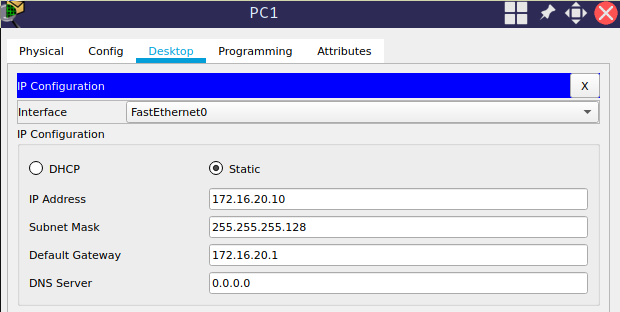
\includegraphics[width=.45\linewidth]{Figures/2020-01-23-133636_620x312_scrot.png}}\hfill
\subfloat[PC2 assign]{\label{Assign3PC2}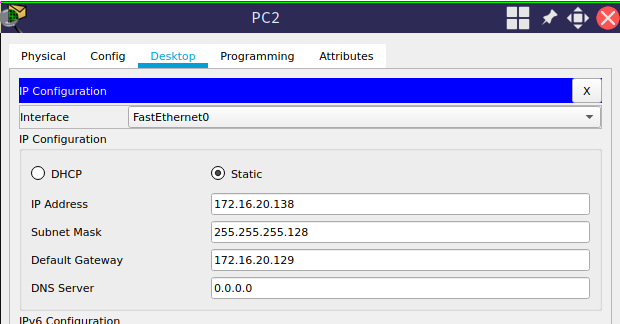
\includegraphics[width=.45\linewidth]{Figures/2020-01-23-133858_620x324_scrot.png}}\par 
\caption{Assigning IPv4 addressing}
\label{Assign3}
\end{figure}


\noindent \\I opened up PC1 and clicked on the desktop. I then opened the
IPconfiguration box and entered the Information from the table. See
Fig~\ref{Assign3}\subref{Assign3PC1}.
\hfill\break

I opened up PC2 and clicked on desktop and opened the ipconfiguration box and entered
the information from the table. See Fig~\ref{Assign3}\subref{Assign3PC2}.
\hfill\break

\begin{figure}[!b]\centering
\subfloat[R1 assign]{\label{connect3V4R1}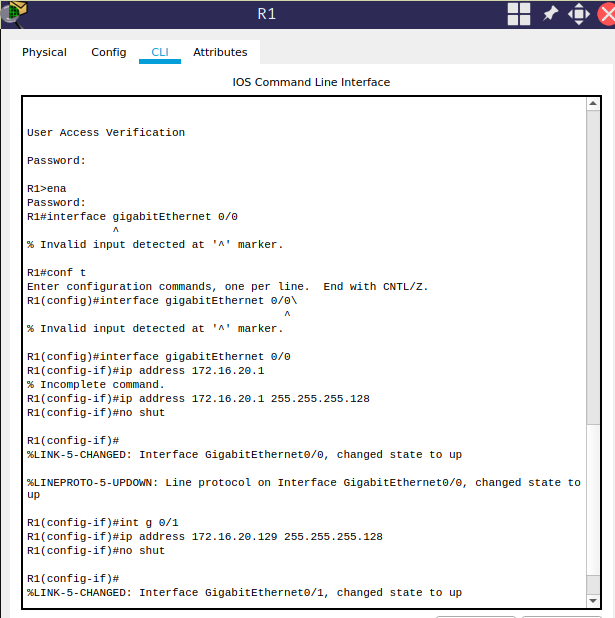
\includegraphics[width=.45\linewidth]{Figures/2020-01-23-134942_615x618_scrot.png}}\hfill
\subfloat[Connected Network Layout]{\label{connect3V4layout}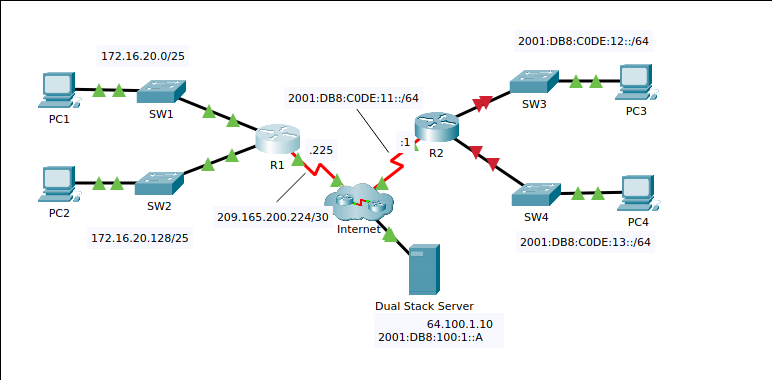
\includegraphics[width=.45\linewidth]{Figures/2020-01-23-135023_772x380_scrot.png}}\par 
\caption{Network Connectivity}
\label{connect3V4}
\end{figure}


\noindent \\I opened up R1 and and used the commandline tool to enter the information
according to the chart. See Fig~\ref{connect3V4}\subref{connect3V4R1}.
\hfill\break

We can now see that PC1 PC2 and R1 are all connected to each other. See
Fig~\ref{connect3V4}\subref{connect3V4layout}.
\hfill\break

\newpage

\noindent\mysubsection{2}{Verify connectivity}
\\I opened PC1 went the command line and successfully pinged the Dual stack server and
then successfully pinged PC2. See Fig~\ref{verify3V4}\subref{verify3V4PC1}
\\I opened PC2 went the command line and successfully pinged the Dual stack server and
then successfully pinged PC1 See Fig~\ref{verify3V4}\subref{verify3V4PC2}

\hfill\break

\begin{figure}[!hbt]\centering
\subfloat[PC1 Successfully pinging the server and PC2]{\label{verify3V4PC1}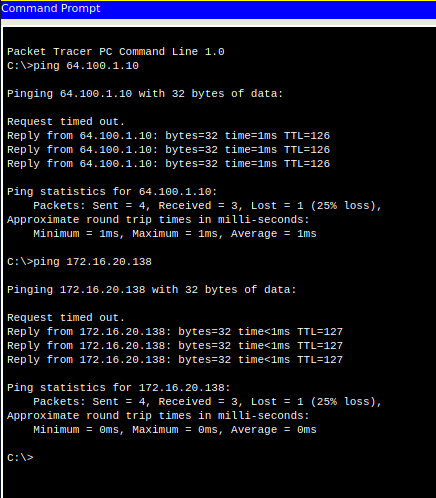
\includegraphics[width=.44\linewidth]{Figures/2020-01-23-135818_436x498_scrot.png}}\hfill
\subfloat[PC2 successfully pinging the server and PC1]{\label{verify3V4PC2}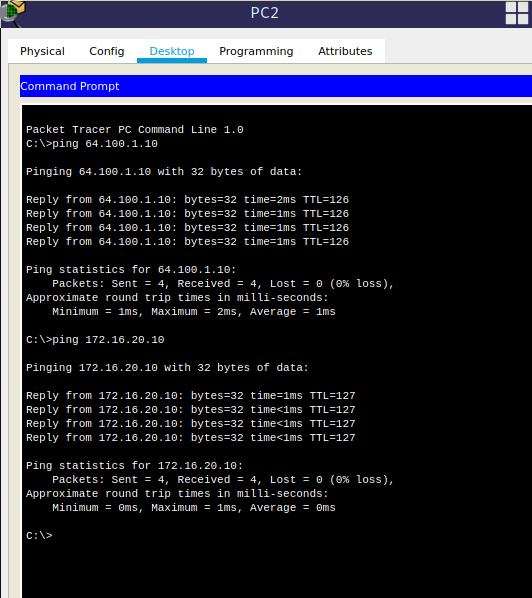
\includegraphics[width=.45\linewidth]{Figures/2020-01-23-135928_532x598_scrot.png}}\par 
\caption{Network Verification}
\label{verify3V4}
\end{figure}


\newpage

%===================================
\mysection{Part 2: configuring IPv6}

\begin{figure}[!hbt]\centering
\subfloat[IPv6 Configuration for PC3]{\label{config3V6PC3}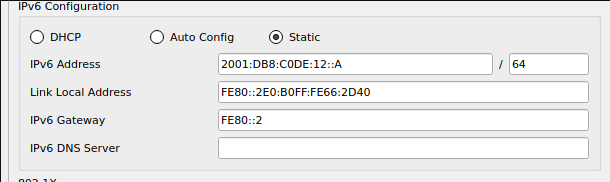
\includegraphics[width=.46\linewidth]{Figures/2020-01-23-142638_610x182_scrot.png}}\hfill
\subfloat[IPv6 Configuration for PC4]{\label{config3V6PC4}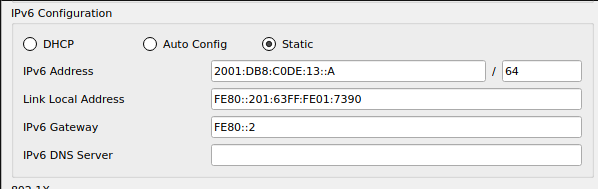
\includegraphics[width=.45\linewidth]{Figures/2020-01-23-142659_598x189_scrot.png}}\par 
\subfloat[Configuring R2 Interface]{\label{config3V6R2}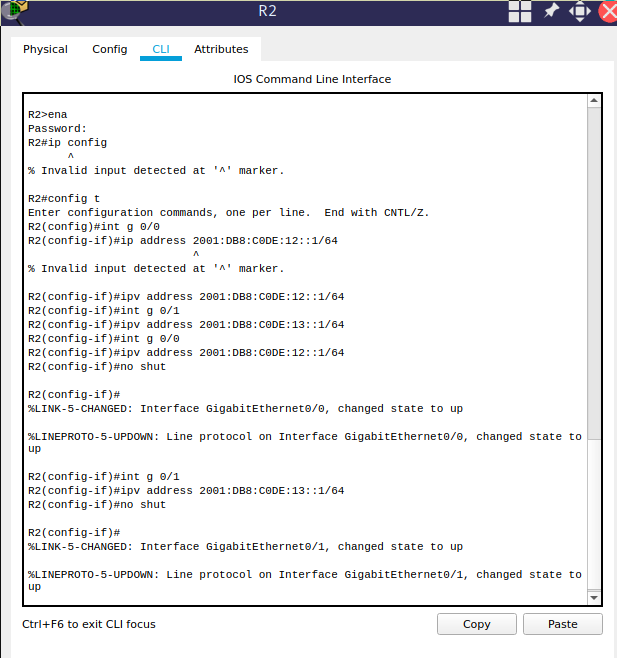
\includegraphics[width=.40\linewidth]{Figures/2020-01-23-141350_617x658_scrot.png}}\hfill
\subfloat[PC3 PC4 and R2 Connections]{\label{config3V6layout}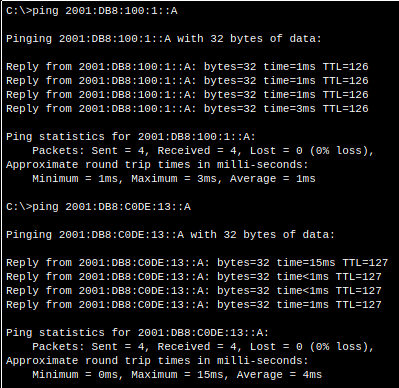
\includegraphics[width=.44\linewidth]{Figures/2020-01-23-142804_399x388_scrot.png}}\par 
\caption{IPv6 Configuration}
\label{config3V6}
\end{figure}

\noindent\mysubsection{1}{Assign IPv6 addressing and verify connectivity}
\\I opened up PC3 and clicked on desktop and opened the ipconfiguration box and
entered the information from the table. See Fig~\ref{config3V6}\subref{config3V6PC3}.

\hfill\break

I opened up PC4 and clicked on desktop and opened the ipconfiguration box and entered
the information from the table. See Fig~\ref{config3V6}\subref{config3V6PC4}

\hfill\break

I opened up R2 and and used the commandline tool to enter the information according to
the chart. See Fig~\ref{config3V6}\subref{config3V6R2}.

\hfill\break

We can now see in Fig~\ref{config3V6}\subref{config3V6layout} that PC3 PC4 and R2 are all connected to each other. 

\clearpage

\noindent\mysubsection{2}{Verify connectivity}
\\I opened PC3 went the command line and successfully pinged the Dual stack server and then successfully pinged PC4

\begin{figure}[!hbt]\centering
  \subfloat[Pinging the Server and PC4 from PC3]{\label{Verify3V6PC3}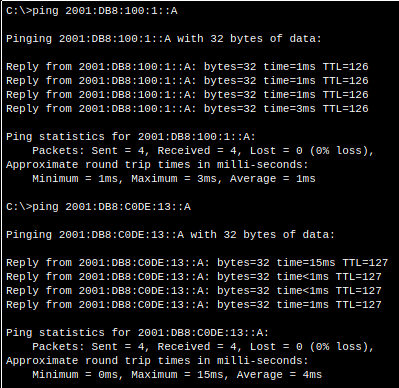
\includegraphics[width=.46\linewidth]{Figures/2020-01-23-142804_399x388_scrot.png}}\hfill
  \subfloat[Pinging the Server and PC3 from PC4]{\label{Verify3V6PC4}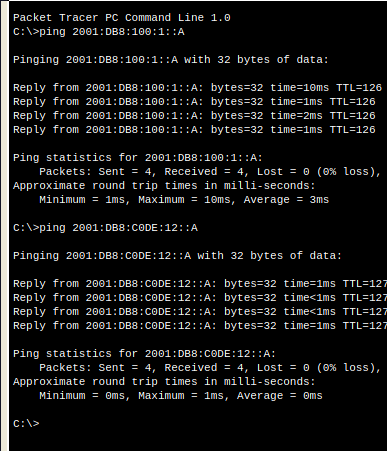
\includegraphics[width=.45\linewidth]{Figures/2020-01-23-142902_387x451_scrot.png}}\par
  \subfloat[Topology of the Completed Network]{\label{Verify3V6Topology}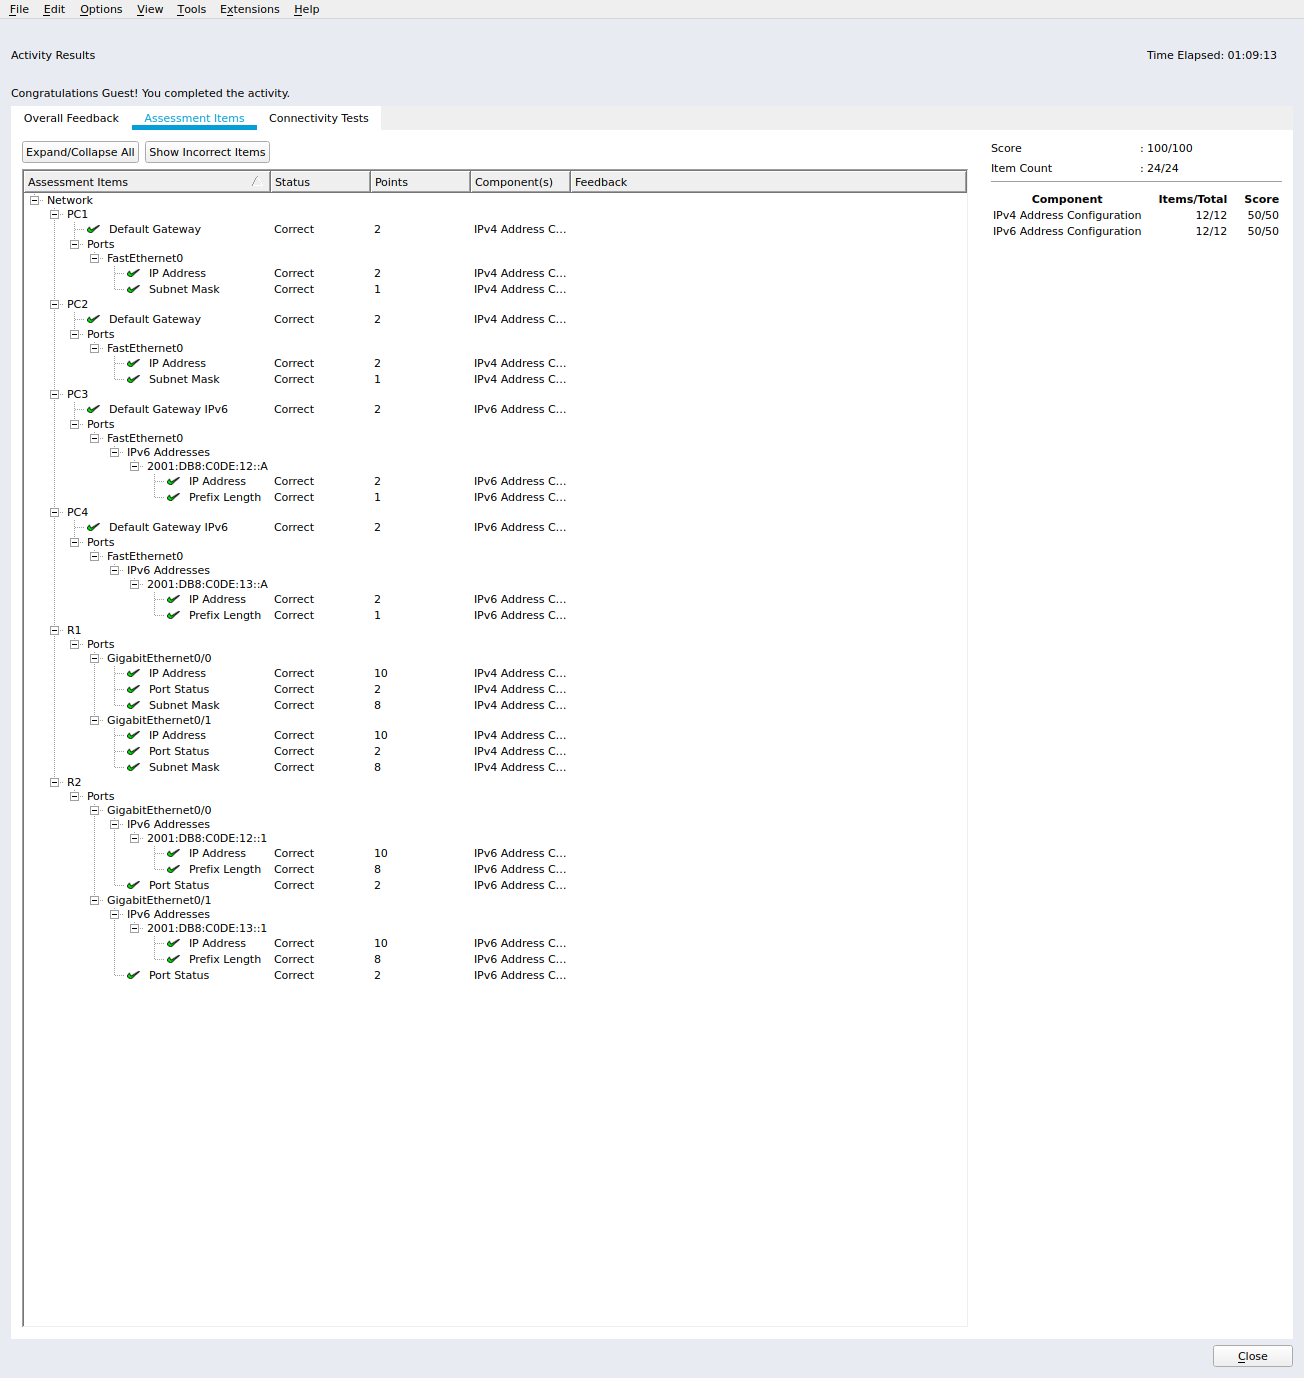
\includegraphics[width=.45\linewidth]{Figures/2020-01-23-143037_1304x1378_scrot.png}}
  \caption{Verifying Connectivity of the Network}
  \label{Verify3V6}
\end{figure}

I opened PC4 went the command line and successfully pinged the Dual stack server and then successfully pinged PC3
\begin{center}
	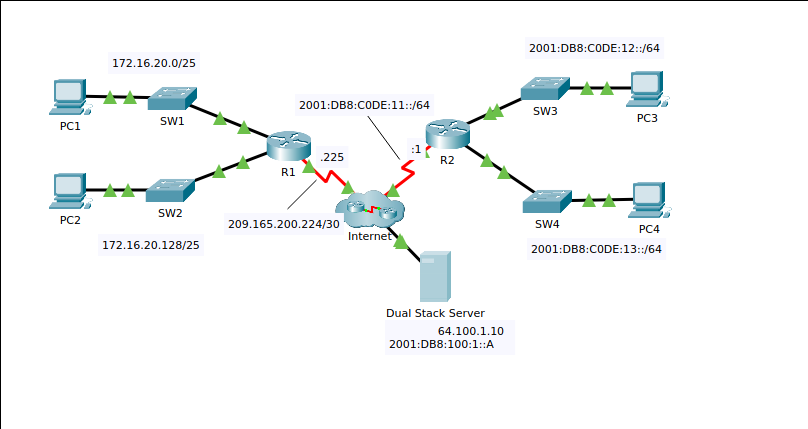
\includegraphics[scale=0.4]{Figures/2020-01-23-142952_808x429_scrot.png}
\end{center}

\newpage

%===================================
\mysection{Part 3: Wrap Up}

\mysubsection{1}{Success}
\\Clicked the Check results button 100\% success
\begin{center}
	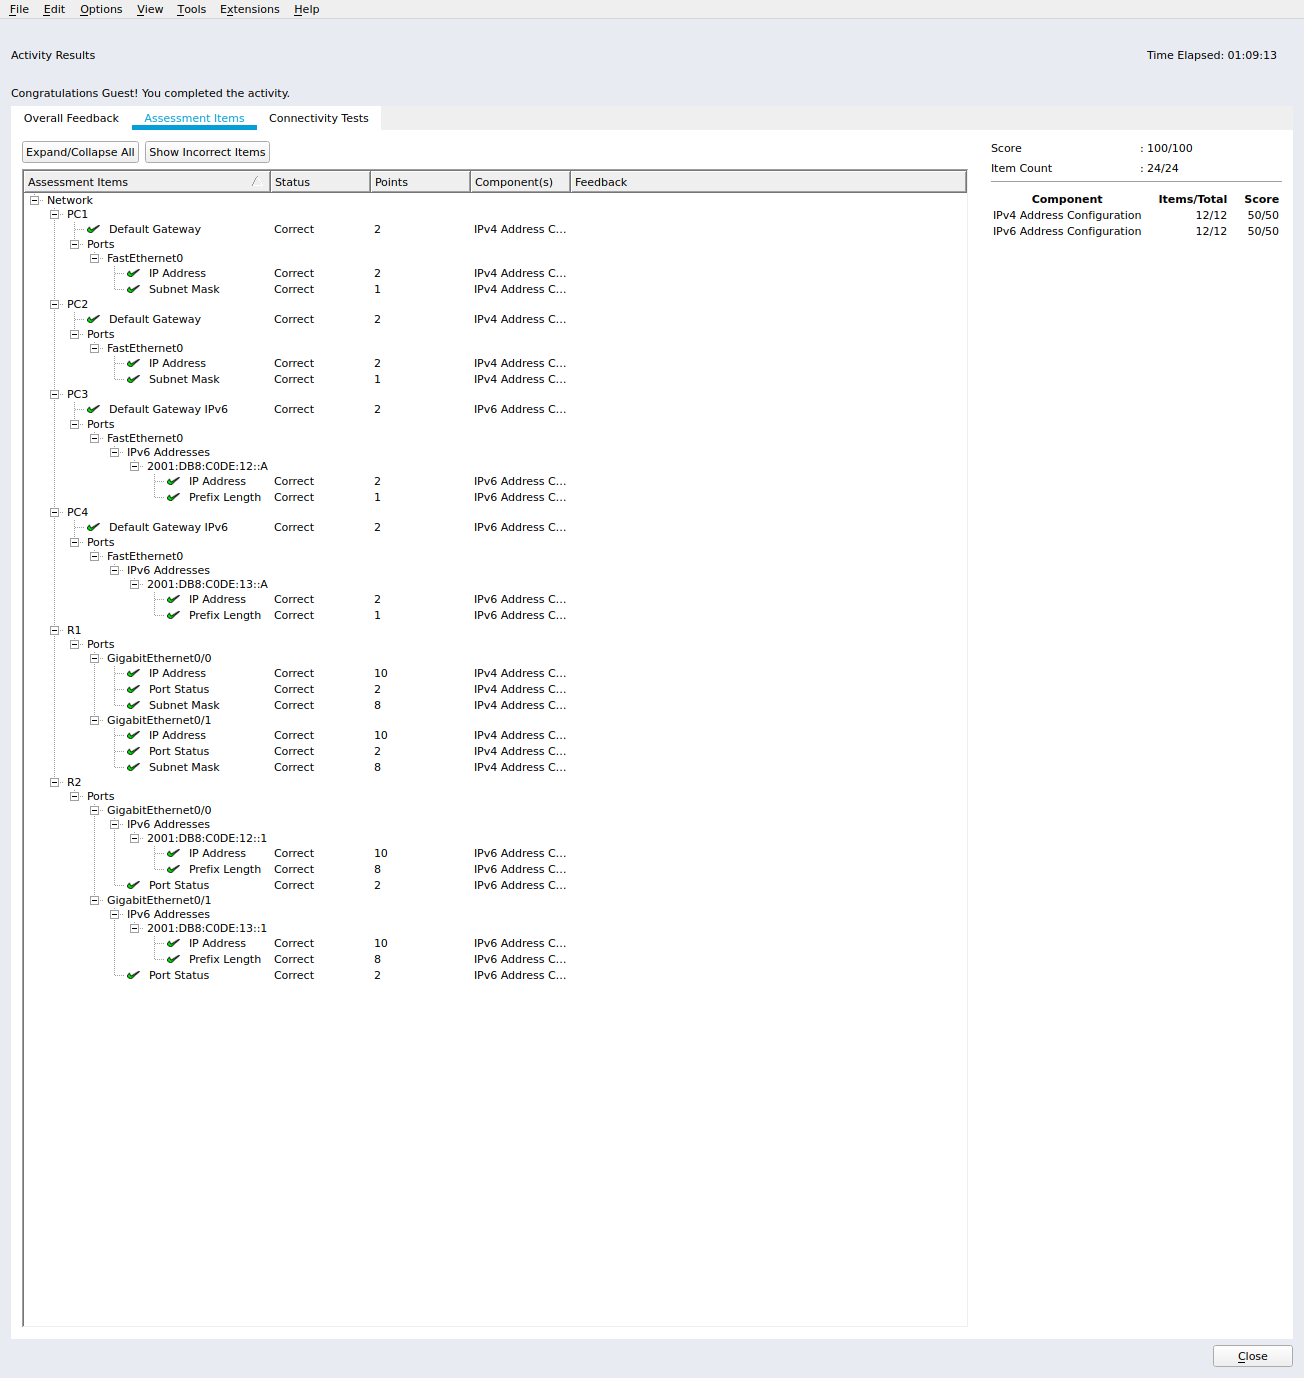
\includegraphics[scale=0.30]{Figures/2020-01-23-143037_1304x1378_scrot.png}
\end{center}

\end{document}

